


% This LaTeX was auto-generated from an M-file by MATLAB.
% To make changes, update the M-file and republish this document.






  
    

\section{Genetic Algorithm Tester} \label{sec:GenAlgTests}
This script file tests the function GenAlg.m program, a module in the SSA
program. The program will be tested for the relative error of the
critical factor of safety for an example slip compared to the critical
factor of safety from a paper analyzing the same example slip. Repeated
analysis of an example slip will also be performed to analyze the
consistency of the algorithm.

\subsection{Example 1}
Comparing results for the example from Greco (1996), Malkawi et al
(2001), Cheng et al (2007), Li et al (2010).

\subsubsection{Consistency Testing}
Firstly this example is used as a method of testing the consistency of
the implemented genetic algorithm. Using the same input for the genetic
algorithm to solve for the critical slip surface 15 times the physical
and critical factor of safety range the algorithm generates as critical
clip surfaces will be investigated.

For each solution a second order polynomial is fit to the vertexes
describing that solutions critical slip surface. The approximately
quadratic shape of the slip surface makes a second order polynomial an
appropriate fit. Solutions are of the form:
\[ y(x) = C_{\text{1}} \cdot x^2 + C_{\text{2}} \cdot x + C_{\text{3}} \]
Where $y$ is the vertical height of the slip surface at horizontal point
$x$. The following histograms show the spread of the fitting constants
$C_\text{1}$, $C_\text{2}$, and $C_\text{3}$. If the algorithm is
consistent the slip surfaces will follow similar shapes and the
constants will have little spread.


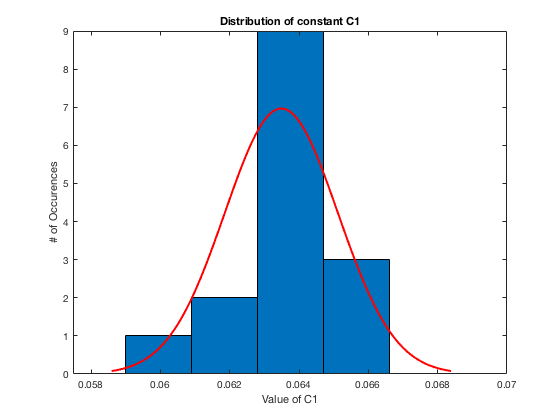
\includegraphics [width=5in]{./VV_SubDocuments/SSA_GenAlgTester_01.png}




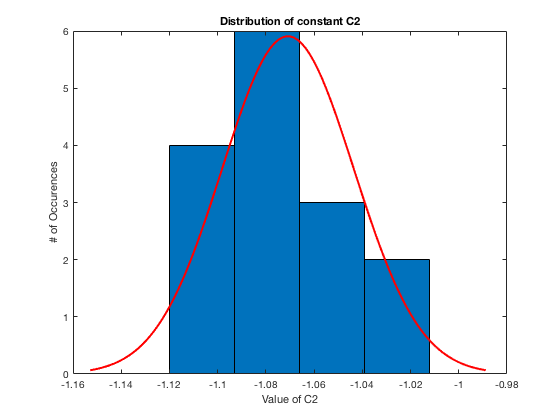
\includegraphics [width=5in]{./VV_SubDocuments/SSA_GenAlgTester_02.png}




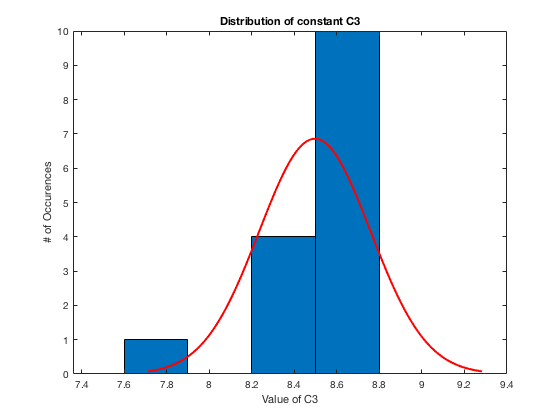
\includegraphics [width=5in]{./VV_SubDocuments/SSA_GenAlgTester_03.png}



The results in the figures show that the normal distribution of results
is approximately followed with few outlying data points, and that the
spread of the constants for the different fits is small, differing over a
small range. This suggests a consistent solution.

        
\color{lightgray} \begin{verbatim}
C1 has a standard deviation of 0.00
C2 has a standard deviation of 0.03
C3 has a standard deviation of 0.26
\end{verbatim} \color{black}
    

The next figure shows a plot of all the critical slip surfaces generated,
supporting the previous findings by showing all the slip surfaces
existing along a narrow band. The band width was measured at the entry
and exit points of the slope for context.

        
\color{lightgray} \begin{verbatim}
The entry band width was : 0.982
The exit band width was : 1.402

\end{verbatim} \color{black}
    

        
\color{lightgray} \begin{verbatim}
Undefined function or variable 'nlayer'.

Error in SSA_GenAlgTester (line 177)
for ilayer=1:nlayer % loop through layers

\end{verbatim} \color{black}
    

The previous results demonstrate that the algorithm generates spatially
consistent solutions. The consistency of the Factor of Safety for the
critical slips surface will now be investigated.  The following histogram
summarizes the distribution of calculated critical factors of safety. The
figure shows a consistent factor of safety calculation, with results
differing over a small range.

The following figure shows the progression of the critical slip factor of
safety over each generation of the genetic algorithm. The red dot
represents the final generation. The figure generally shows convergence
after approximately 130 generations. All solutions also seem to follow
the same general path to convergence.

The results seen in this section all suggest that the genetic algorithm
can consistently converge to a common critical slip, with a common
critical factor of safety.

\subsubsection{Error Test}
The Example 1 slope problem will now be measured for accuracy based on
the difference between results generated by the algorithm, and results
found scientific papers that analyzed the same example slope. A
comparison between the slip surfaces and factors of safety is made. For
this example the average of all generated slip surfaces was used.
\newline\newline\noindent
The accuracy of the slip is shown visually with a plot, and also
measured using a \textit{distance error} metric. The metric slices the
calculated slip surface, and comparison slip surface equally into 10
description vertexes. The average of distance between vertexes of the
same indice, is then considered the \textit{distance error}.
\newline\newline\noindent
The accuracy of the factor of safety is measured based on relative error
with the comparison factor of safety.

\subsection{Examples 2-7}
Examples 2-7 compare critical factor of safety results for the program to
the results of many different papers. The tables show that results are
very accurate compared to the results in the paper, with a relative
factor of safety errors generally less than 5\% for at least one of the
comparison slips. The plots of the slip surfaces also show a critical
slip that is reasonably similar to the comparison slips.
\newline\newline\noindent
The only exception comes in Example 6. Approximately half the time a
critical factor of safety equal to the result in the paper will be
calculated, while the other half a factor of safety of approximately 0.6
will be calculated. Further investigation of this is found in
\ref{sec:Ex6Tests}.

\subsubsection*{Example 2}
\textbf{Papers:} Zolfaghari et al (2005), Cheng et al (2007),
Li et al (2010)

\subsubsection*{Example 3}
\textbf{Papers:} Zolfaghari et al (2005), Cheng et al (2007),
Li et al (2010)

\subsubsection*{Example 4}
\textbf{Papers:} Cheng et al (2007), Li et al (2010)

\subsubsection*{Example 5}
\textbf{Papers:} Pham and Fredlund (2003), Li et al (2010)

\subsubsection*{Example 6}
\textbf{Papers:} Pham and Fredlund (2003), Li et al (2010)

\subsubsection*{Example 7}
\textbf{Papers:} Fredlund and Krahn (1977)
